\documentclass[a4paper]{article}

\usepackage[english]{babel}
\usepackage[utf8]{inputenc}
\usepackage{amsmath}
\usepackage{graphicx}
\usepackage[colorinlistoftodos]{todonotes}

\usepackage{ragged2e}

\title{
FRT090  \\
Feedback Seminar 2\\}
\author{Group B}

\date{\today}



\begin{document}
\maketitle



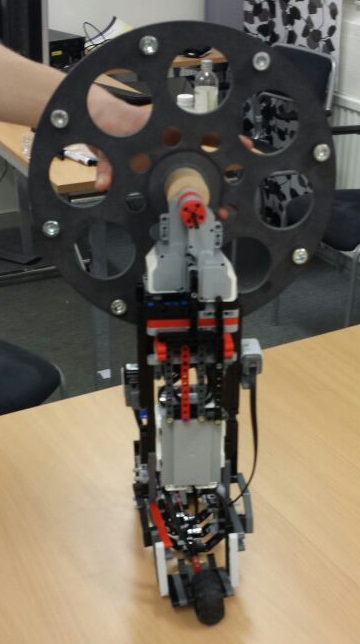
\includegraphics[width=0.7\textwidth]{inwheel}

\newpage

\section{Introduction}

We are designing a unicycle made by lego with an integrated inertia wheel to keep the lateral balence. The project therefore consists of two problems. To stabilize the unicycle in the medial direction by designing a controller for the ground wheel, and to stabilize it in the lateral direction by applying a reaction wheel connected to the top of the unicycle.

\section{Design}

\subsection{Inertia wheel}

We realized early in the project that controlling the inertia wheel is the most complicated part of the project. The complexity comes from several areas. The sensors have to be very accurate (which they are not), the simulation in simulink had to take account of the relationship between torque and the speed of the wheel among other things, we had to design a working controller.

The unicycle is similar to an inverted pendulum with a point mass in the center of mass, with an additional mass that is the inertia wheel, seen in figure 1. We modeled the pendulum as can be seen in (1). The relevant states from the model are the angle of the pendulum, the the angular velocity of the pendulum and the angular velocity of the inertia wheel. The angular position of the inertia wheel is not important as only the change in angular position affects the torque. Torque is the momentum you get when a vector force is acted on the wheel with a certain radius. The torque acting on the pendulum due to gravity (which makes it fall) must be less that the torque from the inertia wheel (which we can control) for it to be stable. The reaction torque is therefore dependent on the radius of the wheel. The maximum torque of the engine is also limited, so some angles are impossible for the reaction wheel to stabilize.

To optimize the controller we implemented a linear quadratic regulator which minimizes the cost function, seen in (2). The Q matrix determines how much each state will be penalized. Since we want to keep cost function (J) small a large Q will require that the states are small. Q=[q1 0 0; 0 q2 0; 0 0 q3].

\begin{figure}
	\centering
	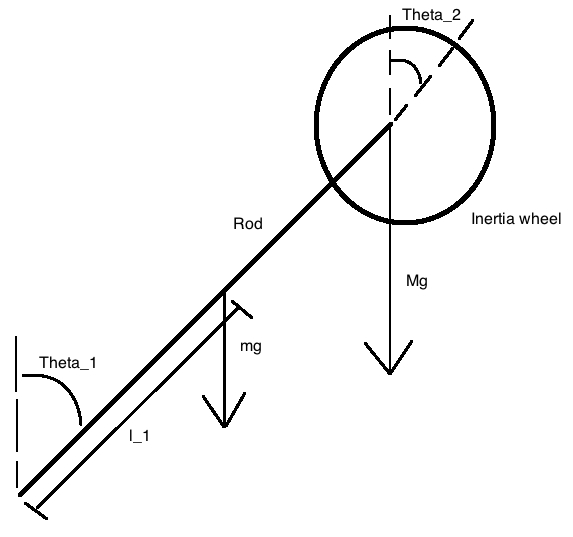
\includegraphics[width=0.7\textwidth]{Inverted_pedulum_2}
	\caption{Shows the sketch of the inverted pendulum}
	\label{fig:sketch_inverted_pendulum}
\end{figure}

\newpage

\begin{equation}
		\begin{aligned}
	     	 (J_{w}+ML^2 + J_{p} ) \frac{\partial^2 \theta_{1} }{\partial t^2}  &= l_{1} \sin{\theta_{1}} m g + L \sin{\theta_{1}} M g - \tau    \\  
		 J_{w} \frac{\partial^2 \theta_{2}} {\partial t^2} &= \tau
		\end{aligned}
	 	\label{equ:inverted_pendulum}  
\end{equation}

\subsubsection{LQR design}

The cost function we needed to minimize was:

\begin{equation}
		\begin{aligned}
	     	 E(x^TQx + u^TRu)
		\end{aligned}
	 	\label{equ:inverted_pendulum}  
\end{equation}


We set the weight matrices to the values:

\begin{itemize}

\item[] q1 = 1/1.57
\item[] q2 = 1/0.349
\item[] q3 = 1/16
\item[] R = 1/0.348

\end{itemize}


These values come from the bounds of the states. The pendulum angle has a range of -1.57 to 1.57 radians (-90 to 90 degrees). We estimated that the maximum speed of the pendulum from free fall is 0.349 rad/s (about 20 degrees per second). The maximum angular velocity of the reaction wheel was determined to be 16 rad/s. Max torque is 0.348 Nm.
These values are used to normalize each product of the cost function so they are approximately equal. These values may need to be tuned, but since the system is not adequately stable there are other problems we need to solve before increasing robustness

In simulink we had to take into account the actuator, being the motor. The torque of the motor rapidly decreases as the speed of the wheel increases. Therefore the max torque could only be achieved at a short time. After several attempts with a PID controller we concluded that with these limitations we had to use state feedback with the cost function shown above.

\subsection{Implementation}



For the state feedback implementation we used  the floating point algorithm, we will not go in to details how the whole implementation process has been made but there are quite important steps in the implenting process which are worthy to be underlined.

To descretize the continouse parameters in the our system we used the zero hold method, 

One problematic issue was that when parameters (the estimated parameters in the model) are changed due to the testing experiments when the model parameteres are changed that is to say the new A and B matrices are dependent on the sampling time (h).


\end{document}